Section~\ref{sec:predictionSection} describes the concepts of prediction within the area of wind production and electricity prices. What is important to emphasize here is the type of input data used for the prediction of both price and production. Meteorological factors are important in both cases and can therefore be extracted from the same source. The second type of data is the prices and the productions themselves. Artificial Neural Networks calculates a generalized function by looking at historical data and comparing with the actual values (Section~\ref{sec:annSection}), e.g. comparing the weather factors at time with the actual production at time. For this reason it is necessary to collect historical meteorological, price and production data in order to do the prediction. A simple drawing of the input and output can be seen in Figure~\ref{fig:verySimpleANN}

\begin{figure}[H]
\centering
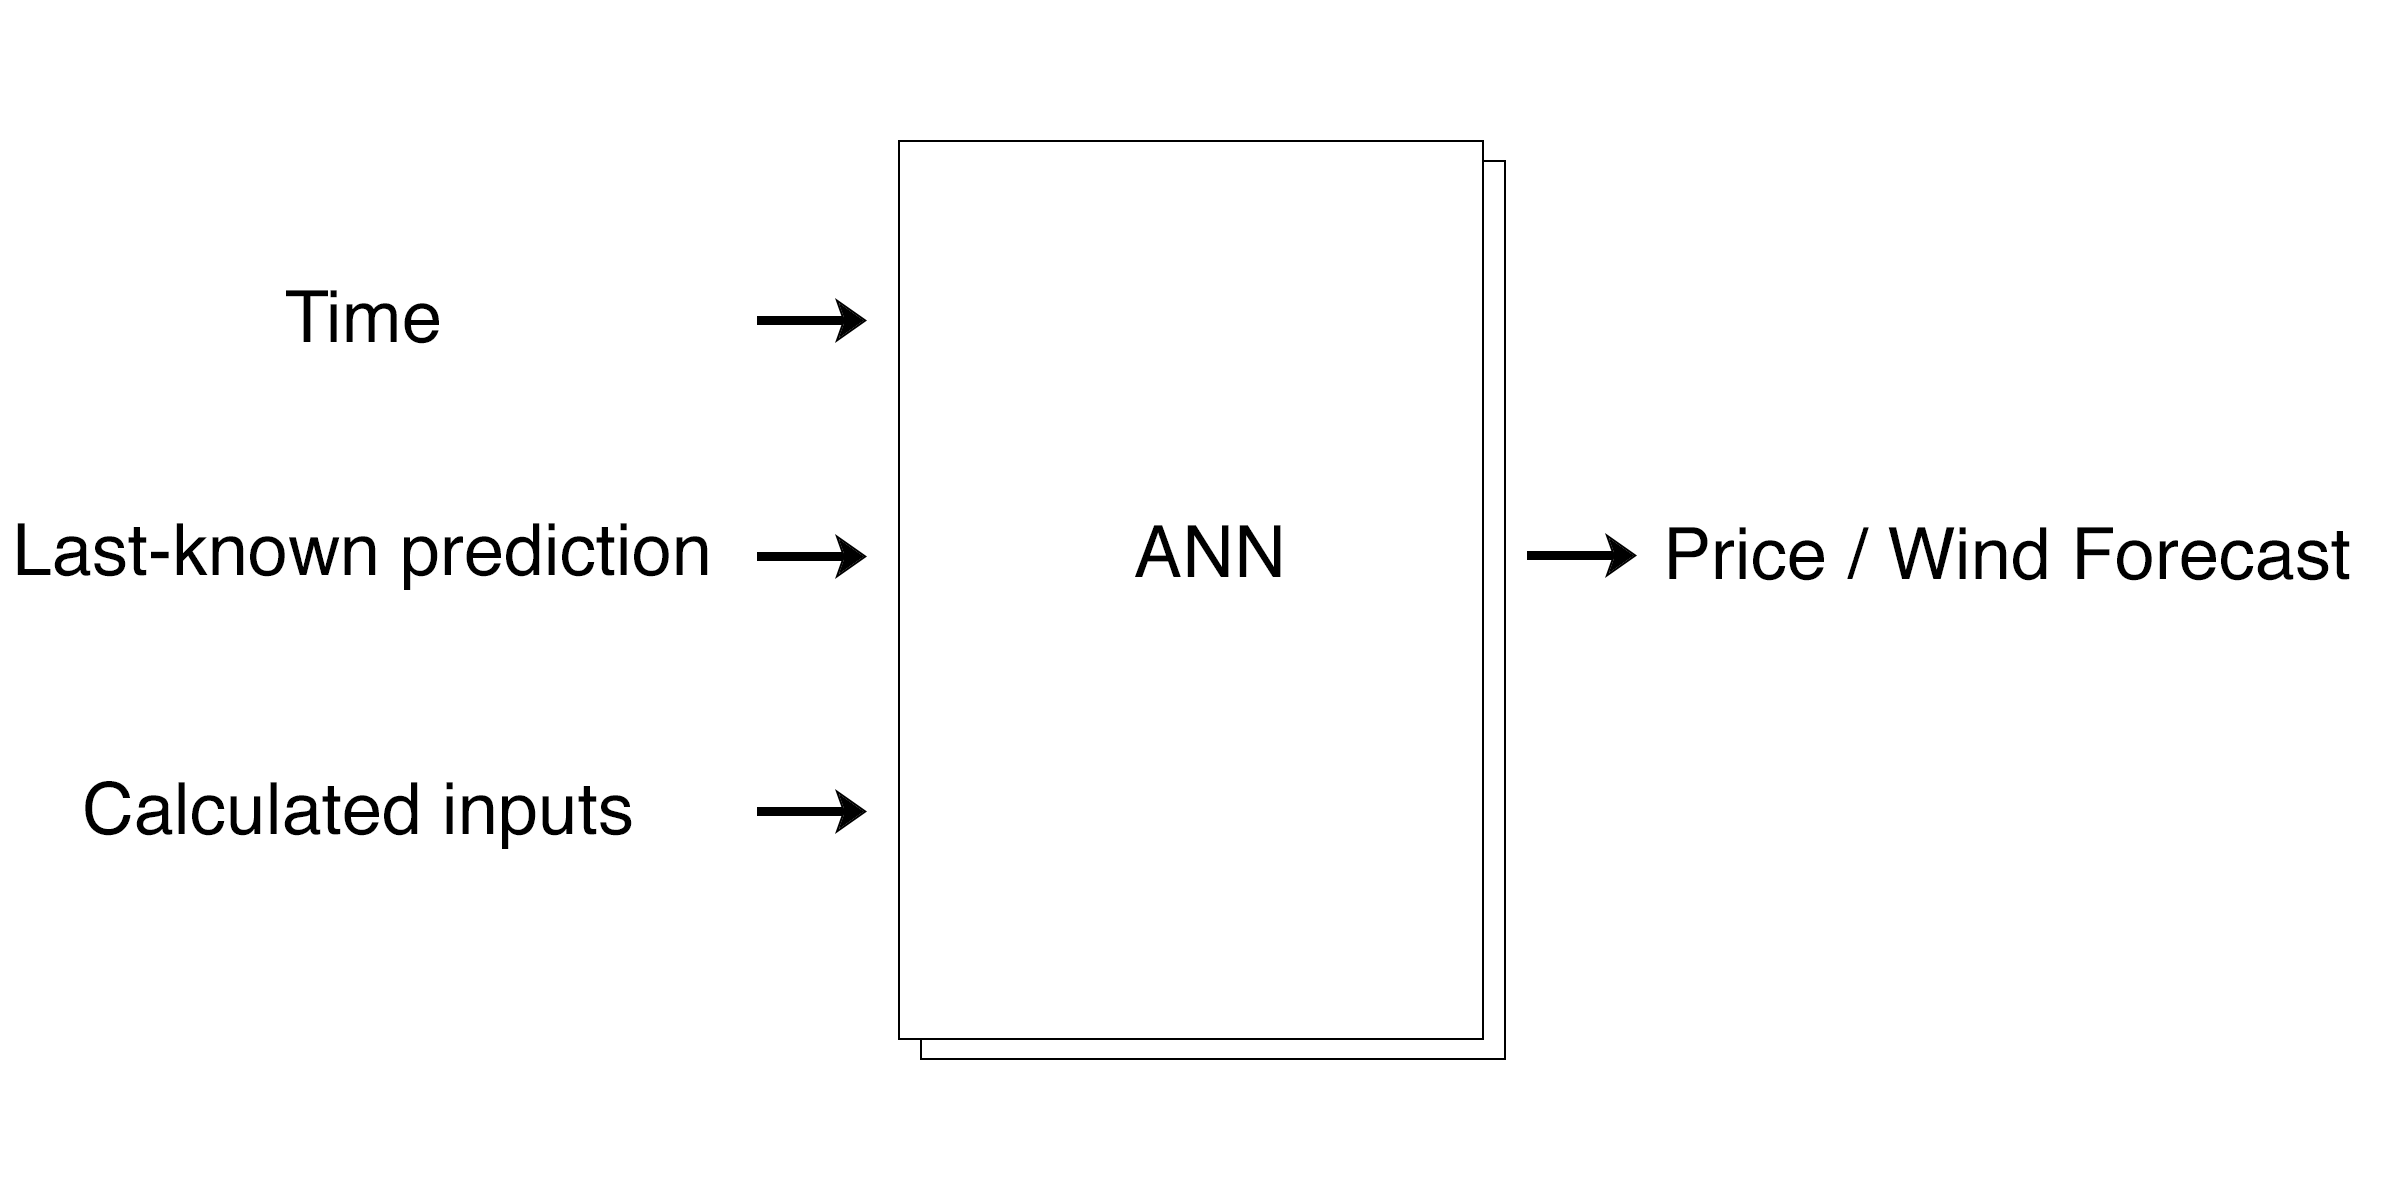
\includegraphics[width=0.85\linewidth]{billeder/simpleANN.png}
\caption{Simple ANN}
\label{fig:verySimpleANN}
\end{figure}

The data must come from a trusted source so that proper predictions can be based on it which is discussed in Section~\ref{sec:uncertainInformation} about uncertain information. The data must be of a certain quality in relation number of observations because we need to make hourly predictions, e.g. the meteorological observations must be within an interval of 60 minutes or else we will ignore data from that particular station.

The National Oceanic and Atmospheric Administration's (NOAA) National Climatic Data Center (NCDC) provides public access to all climate and historical weather data from various weather stations around the world\footnote{\url{http://www.ncdc.noaa.gov/}}. We have used it for collection of historical weather data from various Danish weather stations that delivers observations from at least every hour. The data is in a fixed length format and contains all the necessary weather data for prediction. Format can be seen in Appendix~\ref{sec:weatherDataFormat}. 
The historical hourly price and wind power data has been downloaded from Nord Pool Spot\footnote{\url{www.nordpoolspot.com}} that is a .csv file containing all prices in DKK and the Wind Power in MWh.
The data will be aggregated into one file that contains the needed input and output parameters for both prediction of price and wind production. The file includes all meteorological factors, prices, consumptions and wind productions from every hour of the last two years. 

For the sake of simplicity we will be focusing on West Denmark and Funen which is also known as DK1 in the electricity market [find ref]. The collected data will be validated through plot diagrams that show and establish the relationships between weather conditions and the power generation/price of DK1.

The weather data is collected from available weather stations in DK1 from NOAA and can be seen in Figure~\ref{fig:stations4average} and more specific deails is in Appendix~\ref{sec:weatherStations} - some stations have been omitted due to missing data. The collected data will be averaged and used as basis for creating training sets to be used as input parameters for the Artificial Neural Networks. It is necessary to average the weather data to get a representative picture for all regions included in DK1 because only one price and production exist for all of DK1. It must be made clear that historical weather forecasts have not been possible to obtain and is therefore not included in any of our datasets but data will look the same and have the same format. Daily weather forecasts are accurate (97\% accuracy in 2012\footnote{DMI - http://www.dmi.dk/nyheder/arkiv/nyheder-2013/97-af-vejrudsigterne-ramte-plet/} and we consider the actual data values to be sufficient for our purpose but of course it must be taken into consideration when evaluating our results.

\begin{figure}[H]
\centering
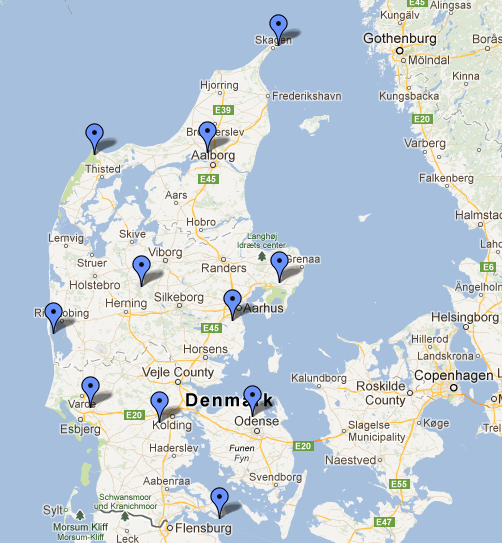
\includegraphics[width=0.85\linewidth]{billeder/stations4average.png}
\caption{Selected weather stations from DK-1}
\label{fig:stations4average}
\end{figure}


We will remove data that is obscure and is related to conditions we cannot predict. (See trimming~\ref{sec:Trimming})

\todo{husk bilag med format}